% Options for packages loaded elsewhere
\PassOptionsToPackage{unicode}{hyperref}
\PassOptionsToPackage{hyphens}{url}
%
\documentclass[
  x11names]{article}
\usepackage{amsmath,amssymb}
\usepackage{lmodern}
\usepackage{iftex}
\ifPDFTeX
  \usepackage[T1]{fontenc}
  \usepackage[utf8]{inputenc}
  \usepackage{textcomp} % provide euro and other symbols
\else % if luatex or xetex
  \usepackage{unicode-math}
  \defaultfontfeatures{Scale=MatchLowercase}
  \defaultfontfeatures[\rmfamily]{Ligatures=TeX,Scale=1}
\fi
% Use upquote if available, for straight quotes in verbatim environments
\IfFileExists{upquote.sty}{\usepackage{upquote}}{}
\IfFileExists{microtype.sty}{% use microtype if available
  \usepackage[]{microtype}
  \UseMicrotypeSet[protrusion]{basicmath} % disable protrusion for tt fonts
}{}
\makeatletter
\@ifundefined{KOMAClassName}{% if non-KOMA class
  \IfFileExists{parskip.sty}{%
    \usepackage{parskip}
  }{% else
    \setlength{\parindent}{0pt}
    \setlength{\parskip}{6pt plus 2pt minus 1pt}}
}{% if KOMA class
  \KOMAoptions{parskip=half}}
\makeatother
\usepackage{xcolor}
\usepackage[margin=1in]{geometry}
\usepackage{graphicx}
\makeatletter
\def\maxwidth{\ifdim\Gin@nat@width>\linewidth\linewidth\else\Gin@nat@width\fi}
\def\maxheight{\ifdim\Gin@nat@height>\textheight\textheight\else\Gin@nat@height\fi}
\makeatother
% Scale images if necessary, so that they will not overflow the page
% margins by default, and it is still possible to overwrite the defaults
% using explicit options in \includegraphics[width, height, ...]{}
\setkeys{Gin}{width=\maxwidth,height=\maxheight,keepaspectratio}
% Set default figure placement to htbp
\makeatletter
\def\fps@figure{htbp}
\makeatother
\setlength{\emergencystretch}{3em} % prevent overfull lines
\providecommand{\tightlist}{%
  \setlength{\itemsep}{0pt}\setlength{\parskip}{0pt}}
\setcounter{secnumdepth}{-\maxdimen} % remove section numbering
\usepackage{fontspec} \usepackage{titling} \pretitle{\begin{center} \vspace{-3cm}
\includegraphics[width=\linewidth]{images/Base_info/logo.png}\LARGE\\} \posttitle{\end{center}} \usepackage{float} \usepackage{fancyhdr} \usepackage{ragged2e} \usepackage{caption} \usepackage{colortbl} \captionsetup[figure]{labelformat=empty} \arrayrulecolor{white} \pagestyle{fancy} \fancyhead[L,C]{} \fancypagestyle{plain}{\pagestyle{fancy}} \PassOptionsToPackage{dvipsnames,svgnames*,x11names*}{xcolor} \definecolor{ceil}{rgb}{0.57, 0.63, 0.81} \usepackage[export]{adjustbox} \usepackage{wrapfig} \usepackage{graphicx} \usepackage{caption}
\usepackage{booktabs}
\usepackage{longtable}
\usepackage{array}
\usepackage{multirow}
\usepackage{wrapfig}
\usepackage{float}
\usepackage{colortbl}
\usepackage{pdflscape}
\usepackage{tabu}
\usepackage{threeparttable}
\usepackage{threeparttablex}
\usepackage[normalem]{ulem}
\usepackage{makecell}
\usepackage{xcolor}
\ifLuaTeX
  \usepackage{selnolig}  % disable illegal ligatures
\fi
\IfFileExists{bookmark.sty}{\usepackage{bookmark}}{\usepackage{hyperref}}
\IfFileExists{xurl.sty}{\usepackage{xurl}}{} % add URL line breaks if available
\urlstyle{same} % disable monospaced font for URLs
\hypersetup{
  hidelinks,
  pdfcreator={LaTeX via pandoc}}

\author{}
\date{\vspace{-2.5em}Fecha de creación: 03 April, 2023}

\begin{document}

\setmainfont{Arial}
\setsansfont{Arial}
\setmonofont{Arial}

\newcommand\invisiblesection[1]{%
  \refstepcounter{section}%
  \addcontentsline{toc}{section}{\protect\numberline{\thesection}#1}%
  \sectionmark{#1}}

\fancyhead[R]{\textbf{http://doi.org/10.31687/SaremLR.19.204}}

%
  \refstepcounter{section}%
  \addcontentsline{toc}{section}{\protect\numberline{\thesection}GENERALIDADES}%
  \sectionmark{GENERALIDADES}
\vspace{-0.4cm}


\includegraphics[width=1\linewidth]{images/Base_info/logo}

\vspace{1cm}

\begin{minipage}{0.7\textwidth}
\vspace{0.3cm}
\fontsize{20}{24}\selectfont\textit{Tayassu pecari}

\vspace{0.3cm}
\fontsize{30}{36}\selectfont Pecarí labiado
\end{minipage}
\hspace{0.05\textwidth}
\begin{minipage}{0.25\textwidth}

\includegraphics[width=\textwidth]{images/en.png}
\end{minipage}

\normalsize

\begin{figure}[H]

{\centering 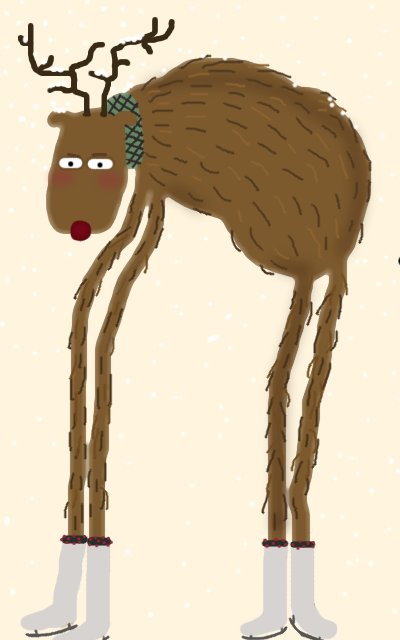
\includegraphics[width=0.35\linewidth]{photos/Blastocerus dichotomus} 

}

\caption{Fotos por Salvador Dali}\label{fig:image}
\end{figure}

\begin{center}\rule{0.5\linewidth}{0.5pt}\end{center}

\justifying

\textbf{Citar como:} de Bustos, Soledad; Varela, Diego; Lizárraga,
Leónidas; Camino, Micaela; Quiroga, Verónica A.. (2019). \emph{Tayassu
pecari}. En: SAyDS--SAREM (eds.) Categorización 2019 de los mamíferos de
Argentina según su riesgo de extinción. Lista Roja de los mamíferos de
Argentina. \url{http://doi.org/10.31687/SaremLR.19.204}

\begin{center}\rule{0.5\linewidth}{0.5pt}\end{center}

\newpage

%
  \refstepcounter{section}%
  \addcontentsline{toc}{section}{\protect\numberline{\thesection}ÁREA DE DISTRIBUCIÓN ACTUAL}%
  \sectionmark{ÁREA DE DISTRIBUCIÓN ACTUAL}
\begin{table}[H]
\centering
\begin{tabular}[t]{>{\raggedright\arraybackslash}m{16cm}>{}m{16cm}}
\toprule
\cellcolor{ceil}{\textcolor{white}{\textbf{\rule{0pt}{14pt}ÁREA DE DISTRIBUCIÓN ACTUAL}}}\\
\bottomrule
\end{tabular}
\end{table}

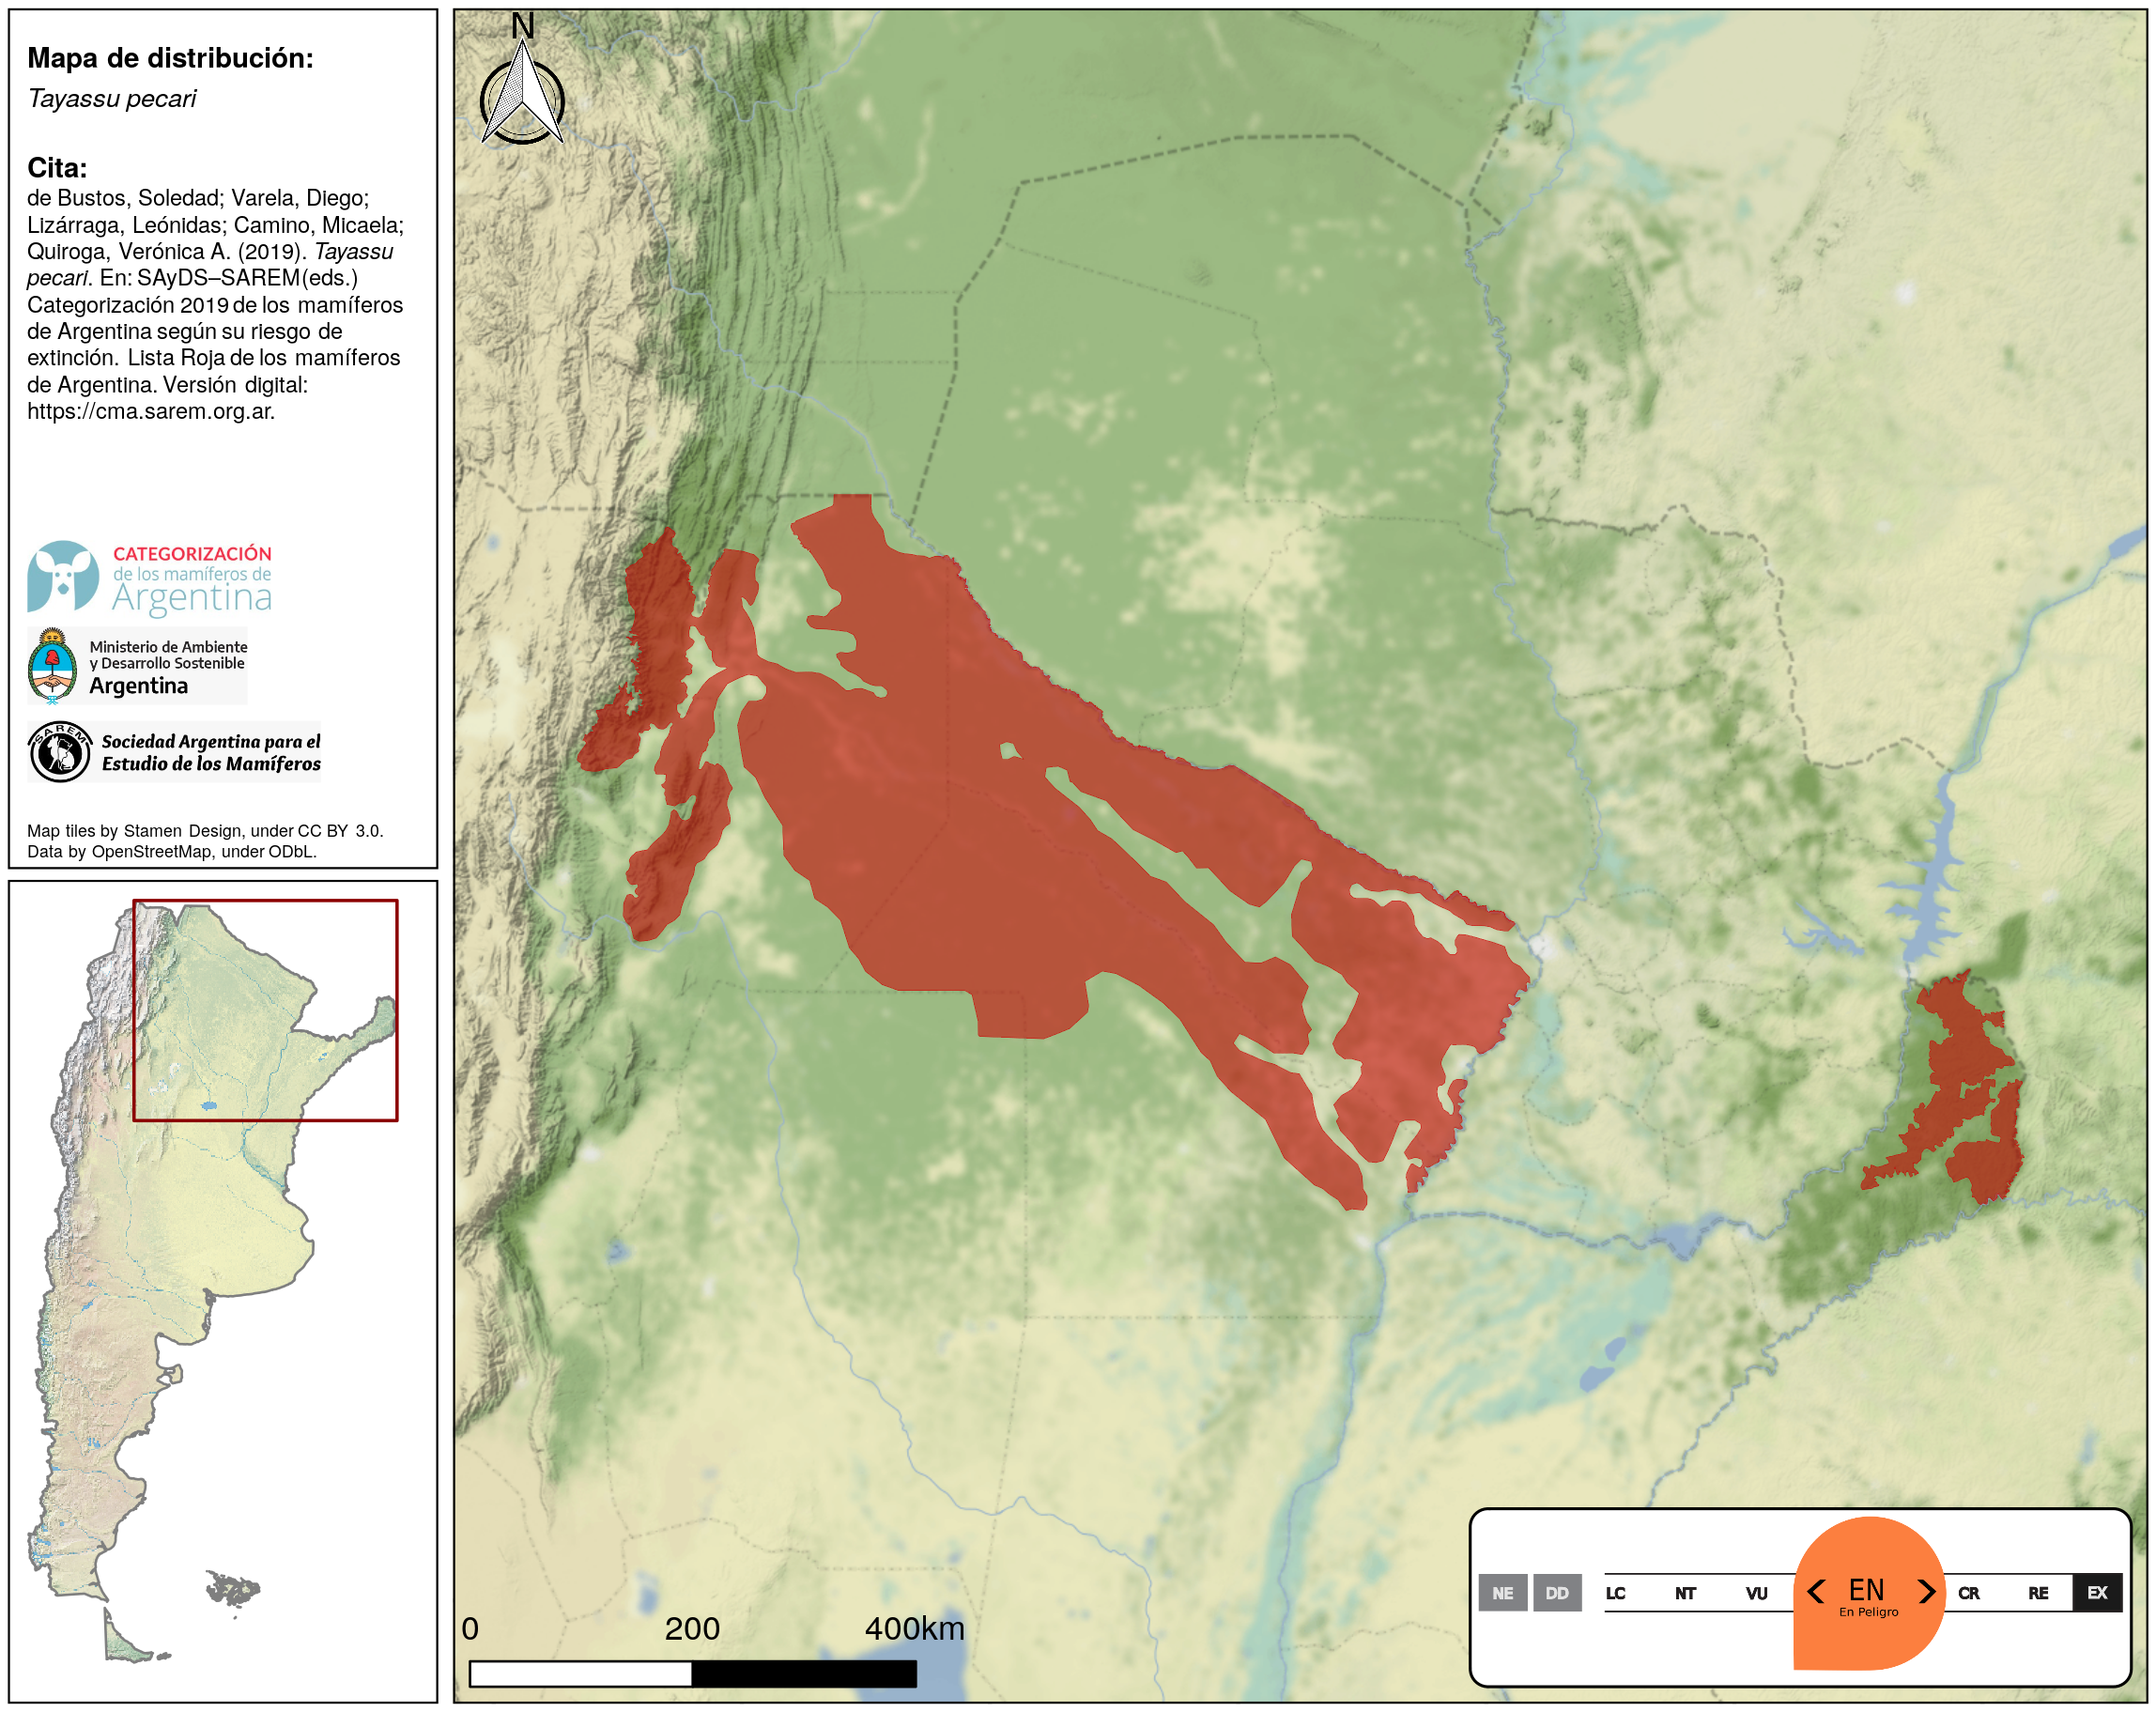
\includegraphics[width=1\linewidth]{maps/Cetartiodactyla/Tayassu_pecari}

%
  \refstepcounter{section}%
  \addcontentsline{toc}{section}{\protect\numberline{\thesection}CATEGORÍAS DE CONSERVACIÓN}%
  \sectionmark{CATEGORÍAS DE CONSERVACIÓN}
\begin{table}[H]
\centering
\begin{tabular}[t]{>{\raggedright\arraybackslash}m{16cm}>{}m{16cm}}
\toprule
\cellcolor{ceil}{\textcolor{white}{\textbf{\rule{0pt}{14pt}CATEGORÍAS DE CONSERVACIÓN}}}\\
\bottomrule
\end{tabular}
\end{table}

\vspace{-0.4cm}

\textbf{Categoría Nacional de Conservación 2019}

EN (En Peligro)

\textbf{Criterios y subcriterios}

A4bcde

\textbf{Justificación de la categorización}

En Argentina el pecarí labiado se distribuye en las ecorregiones de la
Selva Paranaense, el Chaco seco, Chaco húmedo y Yungas, en las
provincias de Jujuy, Salta, Formosa, Chaco, Santiago del Estero y
Misiones, habiéndose extinguido en Tucumán, Catamarca y Corrientes. El
área de distribución abarca alrededor de 172.000 km2, lo que representa
el 25,4 \% de su distribución histórica en nuestro país. En gran parte
de las áreas de ocurrencia, la especie presenta bajas densidades
poblacionales, aunque en áreas óptimas como en áreas protegidas, puede
alcanzar altas densidades. Fue categorizado como En Peligro (EN) dado
que se estima que en las últimas dos generaciones (12 años), la especie
ha sufrido una reducción de la población estimada o inferida de un 50\%
y se sospecha que las amenazas continuarán durante la próxima
generación. Esta reducción es debido a la intensa caza ilegal y la
pérdida de hábitat por la agricultura, ganadería y forestaciones.
También afectan a esta especie, la degradación del hábitat y la
fragmentación de las poblaciones y es posible, que epidemias hayan
llevado al colapso o a fluctuaciones extremas de algunas poblaciones
locales. ~ La problemática de las distintas ecorregiones son diferentes
y desde el punto de vista del manejo hay que tener en cuenta lo
siguiente: ~ - Yungas: la especie sólo está presente en las Yungas de
Salta y Jujuy. En 2009, la sub-población de la Alta Cuenca del Río
Bermejo, fue identificada como la de mayor probabilidad de supervivencia
en Argentina (Taber et al.~2009). Sin embargo, al presente la situación
parece haber cambiado, habiéndose observado una retracción
significativa, llevando a~ la especie casi a su desaparición. Sólo es
posible registrar al pecarí labiado en sitios puntuales, aislados entre
sí y en bajas densidades (Bardavid et al.~2019, de Bustos et al.~2018).
La situación parece ser diferente en la Baja Cuenca del Río Bermejo, en
donde la presencia de la especie es más frecuente (Bardavid et
al.~2019). Ambas subpoblaciones se encuentran escasamente conectadas por
ambientes de transición Yungas-Chaco y por bosques chaqueños. La pérdida
y degradación del hábitat, junto con la cacería ilegal, son las
principales amenazas que enfrenta esta especie y quizás las causas
principales que llevaron a la extinción en Tucumán y Catamarca. Sin
embargo, no se descartan posibles efectos de patógenos que han podido
producir extinciones locales. Sólo es posible registrar al pecarí
labiado en sitios puntuales, aislados entre sí y en bajas densidades
(Bardavid et al.~2019, de Bustos et al.~2018).~ ~ - Chaco: en esta
ecorregión está presente en las provincias de Jujuy, Salta, Chaco,
Formosa y Santiago del Estero. Si bien la extensión de presencia (EOO)
de la especie en la región chaqueña es amplia, sus densidades son bajas
y solo ocurre en sectores con escasa actividad humana (Quiroga 2013;
Perovic et al.~2017; Camino 2016). La especie tiene núcleos
poblacionales importantes en PN El Impenetrable, Estancia~La Leonor y el
Parque Nacional~Río Pilcomayo, siendo muy perseguida para cacería fuera
de estos sitios y de otras áreas protegidas con menores densidades
(Quiroga 2018; Quiroga, V. datos sin publicar). Esta especie es uno de
los mamíferos más perseguidos por su carne en la región chaqueña, por lo
que la cacería intensiva es uno de los principales problemas de
conservación de la especie (Altrichter \& Boaglio 2004; Quiroga 2013).
Actualmente la tasa de pérdida de bosques nativos del Chaco es una de
las más aceleradas del mundo y los procesos de degradación son muy
significativos. Dado que la especie en esta ecorregión se encuentra
asociada a bosques (Altrichter \& Boaglio 2004; Camino 2016), se infiere
una reducción muy alta del tamaño de su población y un futuro incierto
de la misma. ~ - Selva Paranaense: en Misiones, la especie ha
experimentado una reducción de su tamaño poblacional muy alta debido a
la pérdida de hábitat, la cacería y probablemente patógenos, incluyendo
fluctuaciones extremas en sus áreas de ocupación y su abundancia. Entre
1997 y 2008 la especie colapsó en grandes áreas del norte, incluyendo el
P. N. Iguazú (Argentina) y P. N. do Iguacu (Brasil). Actualmente existe
un proceso de recuperación de la especie en estas áreas, pero se infiere
y sospecha, futuras reducciones y fluctuaciones extremas hacia el
futuro. Las causas de estas fluctuaciones no son bien conocidas y se
sospecha que puede estar asociada a algún tipo de patógeno. Las
principales poblaciones de Misiones se encuentran en el bloque norte
(Departamentos de Iguazú y Manuel Belgrano) y en la Reserva de Biosfera
Yabotí (Departamento San Pedro). En la zona centro y sur de la
provincia, si bien la especie está presente, su situación es incierta,
debido a la poca información disponible sobre el estado de sus
poblaciones y la menor cobertura de áreas naturales~ protegidas. La
especie soporta una altísima presión de caza en toda la provincia,
incluso dentro de parques y reservas.

\textbf{Categoría Res. SAyDS 1030/04}

AM (Amenazada)

\textbf{Categorías nacionales de conservación previas (SAREM)}

\arrayrulecolor{white}

%
  \refstepcounter{section}%
  \addcontentsline{toc}{section}{\protect\numberline{\thesection}TAXONOMÍA Y NOMENCLATURA}%
  \sectionmark{TAXONOMÍA Y NOMENCLATURA}
\begin{table}[H]
\centering
\begin{tabular}[t]{>{\raggedright\arraybackslash}m{16cm}>{}m{16cm}}
\toprule
\cellcolor{ceil}{\textcolor{white}{\textbf{\rule{0pt}{14pt}TAXONOMÍA Y NOMENCLATURA}}}\\
\bottomrule
\end{tabular}
\end{table}

%
  \refstepcounter{section}%
  \addcontentsline{toc}{section}{\protect\numberline{\thesection}INFORMACIÓN RELEVANTE PARA LA EVALUACIÓN}%
  \sectionmark{INFORMACIÓN RELEVANTE PARA LA EVALUACIÓN}
\begin{table}[H]
\centering
\begin{tabular}[t]{>{\raggedright\arraybackslash}m{16cm}>{}m{16cm}}
\toprule
\cellcolor{ceil}{\textcolor{white}{\textbf{\rule{0pt}{14pt}INFORMACIÓN RELEVANTE PARA LA EVALUACIÓN}}}\\
\bottomrule
\end{tabular}
\end{table}

%
  \refstepcounter{section}%
  \addcontentsline{toc}{section}{\protect\numberline{\thesection}RANGO GEOGRÁFICO, OCURRENCIA Y ABUNDANCIA Y NOMENCLATURA}%
  \sectionmark{RANGO GEOGRÁFICO, OCURRENCIA Y ABUNDANCIA Y NOMENCLATURA}
\begin{table}[H]
\centering
\begin{tabular}[t]{>{\raggedright\arraybackslash}m{16cm}>{}m{16cm}}
\toprule
\cellcolor{ceil}{\textcolor{white}{\textbf{\rule{0pt}{14pt}RANGO GEOGRÁFICO, OCURRENCIA Y ABUNDANCIA Y NOMENCLATURA}}}\\
\bottomrule
\end{tabular}
\end{table}

%
  \refstepcounter{section}%
  \addcontentsline{toc}{section}{\protect\numberline{\thesection}DATOS MORFOMÉTRICOS}%
  \sectionmark{DATOS MORFOMÉTRICOS}
\begin{table}[H]
\centering
\begin{tabular}[t]{>{\raggedright\arraybackslash}m{16cm}>{}m{16cm}}
\toprule
\cellcolor{ceil}{\textcolor{white}{\textbf{\rule{0pt}{14pt}DATOS MORFOMÉTRICOS}}}\\
\bottomrule
\end{tabular}
\end{table}

%
  \refstepcounter{section}%
  \addcontentsline{toc}{section}{\protect\numberline{\thesection}RASGOS ETO-ECOLÓGICOS}%
  \sectionmark{RASGOS ETO-ECOLÓGICOS}
\begin{table}[H]
\centering
\begin{tabular}[t]{>{\raggedright\arraybackslash}m{16cm}>{}m{16cm}}
\toprule
\cellcolor{ceil}{\textcolor{white}{\textbf{\rule{0pt}{14pt}RASGOS ETO-ECOLÓGICOS}}}\\
\bottomrule
\end{tabular}
\end{table}

%
  \refstepcounter{section}%
  \addcontentsline{toc}{section}{\protect\numberline{\thesection}CONSERVACIÓN E INVESTIGACIÓN}%
  \sectionmark{CONSERVACIÓN E INVESTIGACIÓN}
\begin{table}[H]
\centering
\begin{tabular}[t]{>{\raggedright\arraybackslash}m{16cm}>{}m{16cm}}
\toprule
\cellcolor{ceil}{\textcolor{white}{\textbf{\rule{0pt}{14pt}CONSERVACIÓN E INVESTIGACIÓN}}}\\
\bottomrule
\end{tabular}
\end{table}

%
  \refstepcounter{section}%
  \addcontentsline{toc}{section}{\protect\numberline{\thesection}BIBLIOGRAFÍA}%
  \sectionmark{BIBLIOGRAFÍA}
\begin{table}[H]
\centering
\begin{tabular}[t]{>{\raggedright\arraybackslash}m{16cm}>{}m{16cm}}
\toprule
\cellcolor{ceil}{\textcolor{white}{\textbf{\rule{0pt}{14pt}BIBLIOGRAFÍA}}}\\
\bottomrule
\end{tabular}
\end{table}

\newpage

%
  \refstepcounter{section}%
  \addcontentsline{toc}{section}{\protect\numberline{\thesection}AUTORES}%
  \sectionmark{AUTORES}
\begin{table}[H]
\centering
\begin{tabular}[t]{>{\raggedright\arraybackslash}m{16cm}>{}m{16cm}}
\toprule
\cellcolor{ceil}{\textcolor{white}{\textbf{\rule{0pt}{14pt}AUTORES}}}\\
\bottomrule
\end{tabular}
\end{table}

\textbf{AUTORES}

\begin{tabu} to \linewidth {>{}l>{\raggedright\arraybackslash}p{2cm}>{\raggedright}X}
\toprule
\textbf{\cellcolor{gray!6}{Camino, Micaela}} & \cellcolor{gray!6}{} & \cellcolor{gray!6}{Laboratorio de Biología de la Conservación, Centro de Ecología Aplicada del Litoral (CECOAL) - CONICET, Corrientes, Argentina}\\
\textbf{de Bustos, Soledad} &  & Secretaría de Ambiente y Desarrollo Sustentable de la Provincia de Salta y Fundación Biodiversidad, Salta, Salta, Argentina\\
\textbf{\cellcolor{gray!6}{Lizárraga, Leónidas}} & \cellcolor{gray!6}{} & \cellcolor{gray!6}{Sistema de Información de Biodiversidad (SIB) y Dirección Regional Noroeste, Administración de Parques Nacionales, Salta, Salta, Argentina}\\
\textbf{Quiroga, Verónica A.} &  & Instituto de Diversidad y Ecología Animal (IDEA - CONICET), Centro de Zoología Aplicada, Universidad Nacional de Córdoba - Centro de Investigaciones del Bosque Atlántico (CeIBA), Córdoba, Argentina\\
\textbf{\cellcolor{gray!6}{Varela, Diego}} & \cellcolor{gray!6}{} & \cellcolor{gray!6}{Instituto de Biología Subtropical (IBS), CONICET-Universidad Nacional de Misiones y Centro de Investigaciones del Bosque Atlántico (CeIBA), Puerto Iguazú, Misiones, Argentina}\\
\bottomrule
\end{tabu}

\textbf{COLABORADORES}

\begin{tabu} to \linewidth {>{}l>{\raggedright\arraybackslash}p{2cm}>{\raggedright}X}
\toprule
\textbf{\cellcolor{gray!6}{Bardavid, Sofía}} & \cellcolor{gray!6}{} & \cellcolor{gray!6}{Instituto de Ecorregiones Andinas (INECOA), Universidad Nacional de Jujuy - CONICET, S.S. de Jujuy, Jujuy, Argentina}\\
\textbf{Caruso, María Flavia} &  & Dirección Regional Noroeste-CONICET, Administración de Parques Nacionales y Proyecto Jaguares en el Límite, Salta, Argentina\\
\textbf{\cellcolor{gray!6}{Maras, Gustavo A.}} & \cellcolor{gray!6}{} & \cellcolor{gray!6}{Laboratorio de Ecología Aplicada a la Conservación (LEAC), Facultad de Ciencias Naturales, Universidad Nacional de Salta - CONICET, Salta, Salta, Argentina}\\
\textbf{Perovic, Pablo G.} &  & Dirección Regional Noroeste, Administración de Parques Nacionales y Proyecto Jaguares en el Límite, Salta, Argentina\\
\textbf{\cellcolor{gray!6}{Politi, Natalia}} & \cellcolor{gray!6}{} & \cellcolor{gray!6}{Instituto de Ecorregiones Andinas (INECOA), Universidad Nacional de Jujuy - CONICET - Fundacion CEBio, Jujuy, Argentina}\\
\addlinespace
\textbf{Reppucci, Juan I.} &  & CONICET, Administración de Parques Nacionales, Dirección Regional Noroeste y Proyecto Jaguares en el Límite, Salta, Argentina\\
\textbf{\cellcolor{gray!6}{Rivera, Luis O.}} & \cellcolor{gray!6}{} & \cellcolor{gray!6}{Instituto de Ecorregiones Andinas (INECOA), Universidad Nacional de Jujuy - CONICET - Fundacion CEBio, Jujuy, Argentina}\\
\bottomrule
\end{tabu}

\end{document}
